\documentclass[a4paper,12pt,uplatex,dvipdfmx]{jsarticle}

% 数式
\usepackage{amsmath, amssymb, amsfonts, amsthm}
\usepackage{bm}
% グラフィック
\usepackage{graphicx}
\usepackage{tikz}

\usepackage{url}
\usetikzlibrary{intersections, calc, arrows}

\theoremstyle{definition}
\newtheorem{definition}{定義}
\newtheorem{theorem}{定理}
\newtheorem*{confer}{参考}
\renewcommand{\proofname}{\bf{証明}}

\begin{document}

\title{ガンマ関数とベータ関数について}
\author{@Tdrj2716}
\date{\today}
\maketitle

自分の\LaTeX の練習も兼ね, 有名な関数であるガンマ関数とベータ関数についてまとめました. それぞれ階乗とコンビネーションを正の実数で一般化したものに相当します(実際には実部が正の複素数で定義されます)が, その事実がどのようにして導出できるのかをここでは扱いたいと思います. 定義や性質については高校数学の知識があれば理解は出来ると思いますが, 最後に触れるガンマ関数とベータ関数の間に成り立つ関係式を導出する際に二変数関数の積分の変数変換について知識が必要になります。\\

\begin{definition}[ガンマ関数]
    正の実数$x$について, 次の積分で定義される関数
    \[
        \Gamma(x) = \int_0^\infty t^{x-1}\mathrm{e}^{-t} dt
    \]
    をガンマ関数と呼ぶ. グラフは図~\ref{fig:gamma}のようになる.
\end{definition}

\begin{figure}[ht]
    \begin{center}
        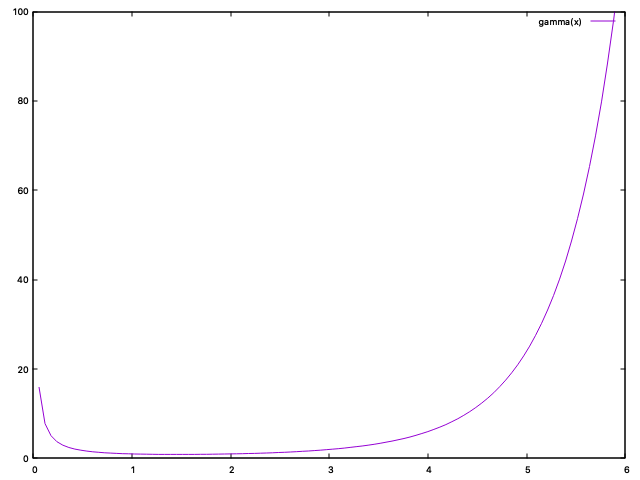
\includegraphics[clip, width=5cm]{gamma.png}
        \caption{ガンマ関数}
        \label{fig:gamma}
    \end{center}
\end{figure}

\newpage
\begin{theorem}[階乗の一般化]
    任意の正整数$n$に対し, 次の式が成り立つ.
    \[
        \Gamma(n+1) = n!
    \]
\end{theorem}
\begin{proof}
    \[
        \Gamma(1) = \int_0^\infty \mathrm{e}^{-t} dt = \lim_{x \to \infty} [-\mathrm{e}^{-t}]_0^x = 1 = 0!
    \]
    また, 任意の正整数$n$に対して
    \begin{align*}
        \Gamma(n) & = \int_0^\infty t^{n-1}\mathrm{e}^{-t} dt = [-t^{n-1}\mathrm{e}^{-t}]_0^{\infty} + \int_0^\infty (n-1)t^{n-2}\mathrm{e}^{-t} dt \\
        & = \lim_{x \to \infty}[-t^{n-1}\mathrm{e}^{-t}]_0^x + (n-1)\int_0^\infty t^{n-2}\mathrm{e}^{-t} dt \\
        & =  0 + (n-1)\Gamma(n-1) 
    \end{align*}
    よって,~$\Gamma(n+1) = n\Gamma(n) = n!\Gamma(1) = n!$. \qedhere\\
\end{proof}
 
\begin{definition}[ベータ関数]
    正の実数$x$, $y$について, 次の積分で定義される関数
    \[
        B(x, y) = \int_0^1 t^{x-1}(1-t)^{y-1} dt
    \]
    をベータ関数と呼ぶ.
\end{definition}

\begin{theorem}[積分公式]
    $m$, $n$が正整数であるとき, 以下の等式が成り立つ.
    \begin{equation}
        B(m, n) = \frac{(m-1)!(n-1)!}{(m+n-1)!}
        \label{eq:b1}
    \end{equation}
    また非負整数$p$, $q$と実数$\alpha$, $\beta(\alpha < \beta)$に対し, 以下の等式が成立する.
    \begin{equation}
        \int_{\alpha}^{\beta}(x-\alpha)^{p}(\beta-x)^{q} dx = \frac{p!q!}{(p+q+1)!}(\beta-\alpha)^{p+q+1}
        \label{eq:b2}
    \end{equation}
\end{theorem}

\begin{proof}
    $n = 1$のときは, $m = 1$で
    \[
        B(1, 1) = \int_0^1 dt = 1
    \] \\
    $m > 1$で
    \[
        B(m, 1) = \int_0^1 t^{m-1} dt = \left[\frac{t^m}{m}\right]_0^1 = \frac{1}{m} = \frac{(m-1)!}{m!}
    \]
    より成り立つ. \\
    $n > 1$のとき, 
    \begin{align*}
        B(m, n) & = \left[\frac{t^m}{m}(1-t)^{n-1}\right]_0^1 + \int_0^1 \frac{t^m}{m}(n-1)(1-t)^{n-2} dt \\
        & = \frac{n-1}{m}B(m+1, n-1)
        = \frac{n-1}{m}\cdot\frac{n-2}{m+1}B(m+2, n-2) = \cdots \\
        & = \frac{(n-1)(n-2)\cdots 1}{m(m+1)\cdots(m+n-2)}B(m+n-1, 1) \\
        & = \frac{(m-1)!(n-1)!}{(m+n-2)!}\cdot\frac{1}{(m+n-1)} \\
        & = \frac{(m-1)!(n-1)!}{(m+n-1)!}
    \end{align*}
    より, 式~(\ref{eq:b1})は示された. \\\\
    また, 式~(\ref{eq:b1})より
    \[
        B(p+1, q+1) = \int_0^1 t^p(1-t)^q dt = \frac{p!q!}{(p+q+1)!}
    \]
    ここで式~(\ref{eq:b2})に対して$x = (\beta - \alpha)t + \alpha$と置換すると, $dx = (\beta - \alpha)dt$, $x:\alpha \to \beta$で$t:0 \to 1$だから
    \begin{align*}
        \int_{\alpha}^{\beta}(x-\alpha)^{p}(\beta-x)^{q} dx
        & = \int_0^1 \{(\beta - \alpha)t\}^p\{(\beta - \alpha)(1-t)\}^q \cdot (\beta - \alpha)dt \\
        & = (\beta - \alpha)^{p+q+1} \cdot B(p+1, q+1) \\
        & = \frac{p!q!}{(p+q+1)!}(\beta-\alpha)^{p+q+1}
    \end{align*}
    より, 式~(\ref{eq:b2})は示された. \qedhere\\
\end{proof}

\begin{confer}
    \[
        \int_\alpha^\beta (x - \alpha)(x - \beta) dx = -\frac{1}{6}(\beta - \alpha)^3,~~ \int_\alpha^\beta (x - \alpha)^2(x - \beta) dx = \frac{1}{12}(\beta - \alpha)^4
    \]
\end{confer}

\newpage
\begin{theorem}
    ベータ関数とガンマ関数の間には次のような関係が成り立つ.
    \[
        B(x, y) = \frac{\Gamma(x)\Gamma(y)}{\Gamma(x + y)}
    \]
\end{theorem}

証明の方針を以下に示す.
\begin{itemize}
    \item 定理1, 2での説明から, $x$, $y$が正整数であるときに成立することは確認出来る.
    \item $x$, $y$が正の実数であるとき,~$\Gamma(x)\Gamma(y) = \Gamma(x + y)B(x, y)$ が成り立つことを(具体的には積分計算する際に極座標に変換する形で)示したい. そのためにまず, ガンマ関数とベータ関数の積分変数を別のものに置き換える.
\end{itemize}

\setcounter{equation}{0}
\begin{proof}
    ガンマ関数
    \[
        \Gamma(x) = \int_0^\infty t^{x-1}\mathrm{e}^{-t} dt
    \]
    に対し,~積分変数$t$を次のように$r$で置換する: $t = r^2~(r \geq 0)$ \\
    このとき,~$dt = 2rdr,~t\colon 0 \to \infty$で$r\colon 0 \to \infty$だから
    \begin{equation}
        \Gamma(x) = \int_0^\infty \mathrm{e}^{-r^2} \cdot r^{2(x-1)} \cdot 2rdr = 2\int_0^\infty \mathrm{e}^{-r^2}r^{2x-1}dr
        \label{eq:gamma}
    \end{equation}
    \newline
    また, ベータ関数
    \[
        B(x, y) = \int_0^1 t^{x-1}(1-t)^{y-1} dt
    \]
    に対し,~積分変数$t$を次のように$\theta$で置換する: $t = \sin^2\theta$ \\
    このとき,~$dt = 2\sin\theta\cos\theta d\theta$,~$t \colon 0 \to 1$で$\theta \colon 0 \to \frac{\pi}{2}$だから
    \begin{align}
        B(x, y) 
        & = \int_0^\frac{\pi}{2} \sin^{2(x-1)}\theta(1-\sin^2\theta)^{y-1} \cdot 2\sin\theta\cos\theta d\theta \nonumber \nonumber\\
        & = 2 \int_0^\frac{\pi}{2} \sin^{2x-1}\theta\cos^{2y-1}\theta d\theta
        \label{eq:beta}
    \end{align}
    
    一方, 式~(\ref{eq:gamma})より,
    \begin{align*}
        \Gamma(x)\Gamma(y)
        & = 2\int_0^\infty \mathrm{e}^{-u^2}u^{2x-1}du \cdot 2\int_0^\infty \mathrm{e}^{-v^2}v^{2y-1}dv \\
        & = 4 \int_0^\infty \int_0^\infty \mathrm{e}^{-(u^2 + v^2)}u^{2x-1}v^{2y-1}dudv
    \end{align*}
    ここで,~積分変数$u$, $v$を$r$, $\theta$で次のように置換する: $u = r\sin\theta,~v = r\cos\theta$ \\
    このときヤコビアンは$r$だから$dudv = rdrd\theta$であり, $r \colon 0 \to \infty,~\theta \colon 0 \to \frac{\pi}{2}$. \\
    よって
    \begin{align*}
        \Gamma(x)\Gamma(y)
        & = 4 \int_0^\infty \int_0^\frac{\pi}{2} \mathrm{e}^{-r^2(\sin^2\theta + \cos^2\theta)}(r\sin\theta)^{2x-1}(r\cos\theta)^{2y-1}rdrd\theta \\
        & = 2 \int_0^\infty \mathrm{e}^{-r^2}r^{2(x+y)-1}dr \cdot 2 \int_0^\frac{\pi}{2} \sin^{2x-1}\theta\cos^{2y-1} d\theta \\
        & = \Gamma(x + y)B(x, y) \hspace{15pt} (式~(\ref{eq:gamma}),~(\ref{eq:beta})より) \\\\
        \therefore B(x, y) & = \frac{\Gamma(x)\Gamma(y)}{\Gamma(x + y)} \qedhere
    \end{align*}
\end{proof}

\begin{thebibliography}{9}
    \bibitem{mathtrain-ガンマ}
    高校数学の美しい物語, ガンマ関数(階乗の一般化)の定義と性質 \\
    \url{https://mathtrain.jp/gamma}
    \bibitem{mathtrain-beta}
    高校数学の美しい物語, ベータ関数の積分公式 \\
    \url{https://mathtrain.jp/beta}
    \bibitem{ガンマ-beta}
    倭算数理研究所, ガンマ関数とベータ関数のよくある関係 \\
    \url{https://wasan.hatenablog.com/entry/20110623/1308805478#%E3%82%AC%E3%83%B3%E3%83%9E%E9%96%A2%E6%95%B0%E3%81%A8%E3%83%99%E3%83%BC%E3%82%BF%E9%96%A2%E6%95%B0%E3%81%AE%E9%96%A2%E4%BF%82%E5%BC%8F}
\end{thebibliography}

\end{document}